\documentclass[10pt,twocolumn,letterpaper]{article}

\usepackage{cvpr}
\usepackage{times}
\usepackage{epsfig}
\usepackage{graphicx}
\usepackage{amsmath}
\usepackage{amssymb}
\usepackage{mathtools}
\graphicspath{ {./images/} }

% Include other packages here, before hyperref.

% If you comment hyperref and then uncomment it, you should delete
% egpaper.aux before re-running latex.  (Or just hit 'q' on the first latex
% run, let it finish, and you should be clear).
\usepackage[breaklinks=true,bookmarks=false]{hyperref}

\cvprfinalcopy % *** Uncomment this line for the final submission

\def\cvprPaperID{****} % *** Enter the CVPR Paper ID here
\def\httilde{\mbox{\tt\raisebox{-.5ex}{\symbol{126}}}}

% Pages are numbered in submission mode, and unnumbered in camera-ready
%\ifcvprfinal\pagestyle{empty}\fi
\setcounter{page}{1}
\begin{document}

%%%%%%%%% TITLE
\title{Perceptron}

\author{Sam Gilbert\\
   a1737770\\}
\maketitle
%\thispagestyle{empty}

%%%%%%%%% ABSTRACT
\begin{abstract}
   The perceptron algorithm is one of the simplest machine learning algorithms. It is a
   form of supervised learning that takes a set of predictor variables and classifies observations
   into a binary class. This report takes an implementation of the Perceptron algorithm and measures
   it performance at classifying observations as either having diabetes or not. Investigations into
   model variability and optimal iteration values were conducted and the impact these have on the
   overall model performance are discussed.
\end{abstract}

%%%%%%%%% BODY TEXT
\section{Introduction}

Perceptron is one of the simplest machine learning algorithms. Perceptron is a supervised learning
algorithm that takes a combination of parameters to make a binary classification. Perceptron was initially
developed in 1958 \cite{cornellProfessorsPerceptron} however was not fully utilised until much later
when it was used in machine learning as a part of multi layer neural networks. The single layer
Perceptron is able to "learn" from a set of information and provide output based on the input information.
Perceptron works by iteratively calculating a set of weights based on the dimension size
of the features in the dataset, $D$. The output of which is a line or $D$ dimension plane
that separates the observations into two categories. Perceptron calculates the updated
weights iteratively and in an ideal world will converge to a $D$ dimension vector of values
that separates all values into their correct groups. Where the data is not able to be
separated cleanly into two groups the Perceptron algorithm will never converge. This requires
a max iteration value to be set such that the problem is bounded. If a max iteration value
is not set the Perceptron algorithm can keep moving back and forth trying to cleanly separate
the training observations into the correct groups. Determining the optimal max iterations
for the dataset will be investigated in the method section of the report.

In this project the Perceptron algorithm was implemented on the Pima Indians Diabetes Database
open source dataset \cite{kagglePimaIndians}. This dataset contains a set of eight medical
predictor variables, the number of pregnancies the patient has had, their BMI, insulin level,
plasma glucose concentration, blood pressure, skin fold thickness, age and their diabetes
pedigree. The dataset also contains an outcome variable which is either the patient has
diabetes or they don't have diabetes. The predictor variables are each one of the $D$
dimensions.
%% talk about activation function

\section{Method}

As outlined in the introduction section the goal of the Perceptron algorithm is to separate
the entries in the dataset into one of two binary groups. The data is read into a python array
of dictionaries with the features being stored in a $D$ dimensional array and the outcome
stored as a signed integer. The data is then split into a training and testing set using the
scikit learn train test function. An 80-20 training testing split was used \cite{gholamy_why_nodate}.

The Perceptron algorithm takes an input layer which is the set of features in each observation, let
the vector of features for observation $i$ be defined as $x_i$. Let the collection of these observations
be defined as $X$. Each of these observations have an outcome variable which is whether the patient has
diabetes or not. Let the outcome for the $i_{th}$ observation be defined as $y_i$. This outcome variable
is either $+1$ if the patient has diabetes or $-1$ if the patient doesn't have diabetes. Let the collection
of all the outcomes for each observation be defined as $Y$. The Perceptron algorithm starts by creating a $D$
dimension vector of weights, defined as $W$. For this implementation the initial $W$ is set as a $D$ dimension
zero vector. A bias value is also required which is defined as $b$ initially set to $0$. This bias shifts the
intercept of the dimensions linear separator away from $0$ and is required as it may not be possible to
split the data points if this doesn't occur.

The Perceptron algorithm works by calculating the dot product of $x_i$ and $W$ and adding the bias, $b$.
The sign function is then passed the result and this is our activation function corresponding to the possible
values of the outcome variable mentioned above. The sign function is defined as

\begin{equation}
   sign(x)= \begin{cases*}
      -1 & if x $<$ 0 \\
      0  & if x = 0   \\
      +1 & if x $>$ 0 \\
   \end{cases*}
\end{equation}

To determine if the perceptron has correctly classified the observation, the result of the sign function
corresponds to the outcome variable possibilities of whether a patient has diabetes or not. Therefore, the
whole process of making a prediction on an observation is defined as.

\begin{equation}\label{eq:pred}
   f(x) = sign((x_i \cdot W) + b)
\end{equation}

Using the predictions from equation \eqref{eq:pred} the weight vector, $W$ can be updated during the training process.
By multiplying the prediction by the actual class of the observation and checking the resulting value is $>0$
the update logic can be simplified. If the result is $>0$ then the perceptron has made a correct prediction
and does not need to be updated. This can be seen in the logic table below showing if a correct
prediction is made the result will always be $>0$ and if an incorrect prediction is made the result will be
$<=0$
\begin{table}[h!]
   \centering
   \begin{tabular}{ ||c c c|| }
      \hline
      Truth & Prediction & Output \\
      \hline
      1     & 1          & 1      \\
      \hline
      1     & -1         & -1     \\
      \hline
      -1    & 1          & -1     \\
      \hline
      -1    & -1         & 1      \\
      \hline
   \end{tabular}      \label{tab:logic}
   \caption{Prediction vs truth logic table for predictions}
\end{table}

If the perceptron makes an incorrect prediction during the training phase $W$ is updated by multiplying
$y_i$ with $x_i$. Let $W$ at the current time be defined as $W_t$. This update step is defined as

\begin{equation}\label{eq:updateweight}
   W_{t+1} = W_t + (y_i * x_i)
\end{equation}

A learning rate value, $\alpha$, can be used when updating $W$ however in the case of the single layer
Perceptron, it does not effect the final result as it will converge on a stable solution regardless. What it
can be used for is altering the volatility of the updates to $W$ and in some cases can speed up the rate at
which the algorithm converges. The equation for updating $W$ that includes the $\alpha$ valu is defined as

\begin{equation}\label{eq:updateweight}
   W_{t+1} = W_t + \alpha (y_i * x_i)
\end{equation}

Similarly, $b$ needs to be updated in the case of an incorrect prediction. Let $b$ at the current time
be defined as $b_t$. The update step is defined as

\begin{equation}\label{eq:updatebias}
   b_{t+1} = b_t + y_i
\end{equation}

This process is repeated for every observation in the training set. In an ideal scenario this process would
be repeated until every element has been correctly classified, however this is most often not possible. Where
the data is not linearly separable on a given dimension the Perceptron algorithm will not be able to converge
on a solution. To address this a max iteration value must be set which will set a stop point for the algorithm
if it fails to converge. This max iteration value is the number of times the algorithm will iterate over the
entire training dataset during the training phase. Different values will be investigated in the results section
to examine the impact it has on the overall model performance.

\section {Results}
\subsection{Max Iteration Investigation}
As discussed above the max iteration value used during the training phase can have a big impact on the
overall model performance. Allowing the model time to converge on an optimal or near optimal solution is
paramount. To determine the appropriate magnitude of the max iteration value, various values were set
during the training phase. A set seed was passed to the function that splits the data into the training
and testing set to ensure each value of max iterations was being tested on the same data.
To reduce the variance in the results,
which will be investigated later, each max iteration value was run 10 times and the mean of the model accuracy
was calculated.
\begin{table}[h!]
   \centering
   \begin{tabular}{ ||c c|| }
      \hline
      Iterations & Mean Accuracy \\
      \hline
      1          & 0.723         \\
      \hline
      10         & 0.730         \\
      \hline
      50         & 0.753         \\
      \hline
      100        & 0.789         \\
      \hline
      500        & 0.703         \\
      \hline
      1000       & 0.703         \\
      \hline
      2000       & 0.736         \\
      \hline
      4000       & 0.730         \\
      \hline
      8000       & 0.697         \\
      \hline
   \end{tabular}      \label{tab:iterations}
   \caption{Iterations vs mean accuracy}
\end{table}

Plotting the results from the table above it can be observed that as the number of max iterations increases,
the corresponding mean accuracy of the Perceptron algorithm also increases before reaching an equilibrium.
For the highest magnitude max iterations the accuracy begins to drop off. This will be investigated in the
discussion section. There is also a spike at the iteration value of 100 and this will be investigated in the
discussion section.
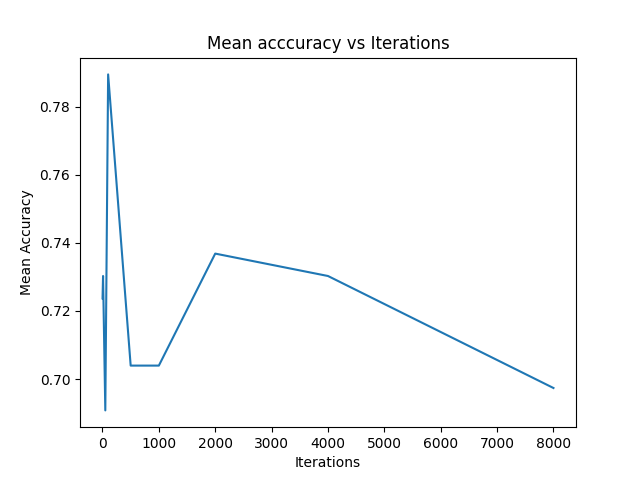
\includegraphics[scale=0.6]{Figure_1.png}
\subsection{Result Variance Investigation}
The variance of the final model accuracy result is highly dependent on the data selected for the training set.
Since the data is randomly selected, the final model $W$ vector and $b$ can vary greatly. The impact of this
was investigated by running the Perceptron algorithm 50 times with an iteration value of 2000 which was found
to provide the best, stable results.

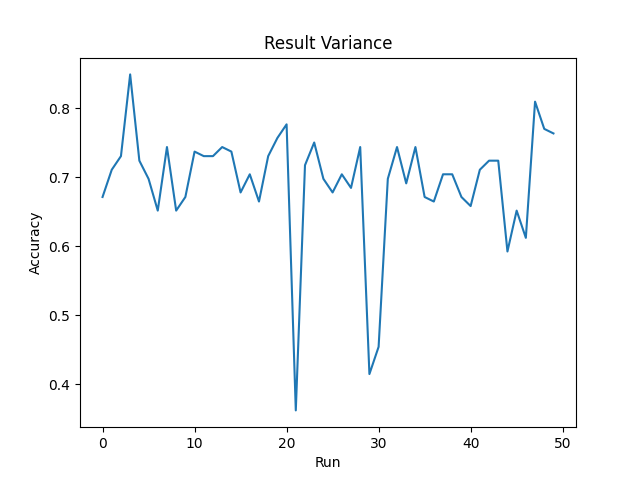
\includegraphics[scale=0.55]{Figure_2.png}
From the plot above it can be observed that the variance of the Perceptron algorithm can vary greatly depending
on the initial split. This can possibly be mitigated and approaches for this will be investigated in the
discussion section

\section{Discussion}
The Perceptron algorithm can be very effective at predicting diabetes using the Pima Indian dataset. Depending
on the number of iterations and the data chosen for the training set accuracy as high as  approximately 0.83
has been observed. It can be highly variable in its performance due to the datasets small size and the lack
of a solution that splits all the observations into the correct groups. With the dataset only containing 768
observations, when it is split into the training and testing sets the training set only contains 614 observations.
This small set of observations leads to variability in the models performance depending on the sample selected.
To address this a bigger dataset could be used which would result in a reduced impact on the final results
caused by the small number of observations.

For this report, outlier data was not accounted for. This could have compounded with the small dataset size
to increase the variability of the final results. If the training dataset contained a high proportion of
observations with outlier data the final $W$ would not result in optimal results when run against the testing
set. Where there is missing data in the observation, the value is set to -1 which does impact the updating
of the $W$ vector. Imputing these values will be discussed in the future work section of this report.

\section{Future Work}
For future work on this problem building a system that trains multiple $W$ vectors and uses the mean of them
as the final value will be investigated. This would reduce the highly variable results caused by the differences
in the training set chosen. It is possible that this could result in the Perceptron overfitting the data
as given enough iterations of the model training it is likely the vast majority of the observations would
be included in one or multiple iterations. The impact of this should be reduced since the weights of a given
observation on the trained model would only be included in a subset of the training iterations. Other future work
would be to address the outlier data through omitting observations that
contain outlier values or devising a method of keeping them out of the training set which would likely
increase the models average performance. Another approach would be to replace the missing values in any
given observation with the mean value of the dataset.

\section{Conclusion}
The Perceptron algorithm performs well at predicting diabetes based on the available variables from the Pima
Indians dataset. With the small dataset available the Perceptron algorithm is able to make predictions with
an average accuracy of approximately 0.75. This result is highly dependant on the subset of the data used
for the training set and an investigation was completed to investigate this. It was found that using this
dataset, the Perceptron was never able to converge on a solution that separated all of the observations into
their correct groups. The impact on model performance from different max iterations was investigated and it
was found that a good balance of variability and performance occured at approximately 2000 iterations.
Strategies were outlined in the future work section of this report for addressing variability present
in the model training process and handling of missing data from some of the observations.
%-------------------------------------------------------------------------
\small
\bibliographystyle{ieee_fullname}
\bibliography{egbib}

\section{Appendix}
Github repository link:  \url{https://github.com/sjg546/COMPSCI7318_Assignment1}

\end{document}
